\documentclass[a4paper,12pt]{extarticle}
\usepackage[utf8x]{inputenc}
\usepackage[T1,T2A]{fontenc}
\usepackage[russian]{babel}
\usepackage{hyperref}
\usepackage{indentfirst}
\usepackage{listings}
\usepackage{color}
\usepackage{here}
\usepackage{array}
\usepackage{multirow}
\usepackage{graphicx}
\usepackage{amsmath}
\usepackage{amssymb}

\usepackage{caption}
\renewcommand{\lstlistingname}{Программа} % заголовок листингов кода

\bibliographystyle{ugost2008ls}

\usepackage{listings}
\lstset{ %
extendedchars=\true,
keepspaces=true,
language=C,						% choose the language of the code
basicstyle=\footnotesize,		% the size of the fonts that are used for the code
numbers=left,					% where to put the line-numbers
numberstyle=\footnotesize,		% the size of the fonts that are used for the line-numbers
stepnumber=1,					% the step between two line-numbers. If it is 1 each line will be numbered
numbersep=5pt,					% how far the line-numbers are from the code
backgroundcolor=\color{white},	% choose the background color. You must add \usepackage{color}
showspaces=false				% show spaces adding particular underscores
showstringspaces=false,			% underline spaces within strings
showtabs=false,					% show tabs within strings adding particular underscores
frame=single,           		% adds a frame around the code
tabsize=2,						% sets default tabsize to 2 spaces
captionpos=t,					% sets the caption-position to top
breaklines=true,				% sets automatic line breaking
breakatwhitespace=false,		% sets if automatic breaks should only happen at whitespace
escapeinside={\%*}{*)},			% if you want to add a comment within your code
postbreak=\raisebox{0ex}[0ex][0ex]{\ensuremath{\color{red}\hookrightarrow\space}},
texcl=true,
inputpath=listings,                     % директория с листингами
}

\usepackage[left=2cm,right=2cm,
top=2cm,bottom=2cm,bindingoffset=0cm]{geometry}

%% Нумерация картинок по секциям
\usepackage{chngcntr}
\counterwithin{figure}{subsection}
\counterwithin{table}{section}

%%Точки нумерации заголовков
\usepackage{titlesec}
\titlelabel{\thetitle.\quad}
\usepackage[dotinlabels]{titletoc}

%% Оформления подписи рисунка
\addto\captionsrussian{\renewcommand{\figurename}{Рис.}}
\captionsetup[figure]{labelsep = period}

%% Подпись таблицы
\DeclareCaptionFormat{hfillstart}{\hfill#1#2#3\par}
\captionsetup[table]{format=hfillstart,labelsep=newline,justification=centering,skip=-10pt,textfont=bf}

%% Путь к каталогу с рисунками
\graphicspath{{fig/}}

\setcounter{tocdepth}{3}

\begin{document}	% начало документа

% Титульная страница
\begin{titlepage}	% начало титульной страницы

	\begin{center}		% выравнивание по центру

		\large Санкт-Петербургский Политехнический Университет Петра Великого\\
		\large Институт компьютерных наук и технологий \\
		\large Кафедра компьютерных систем и программных технологий\\[6cm]
		% название института, затем отступ 6см
		
		\huge Телекоммуникационные технологии\\[0.5cm] % название работы, затем отступ 0,5см
		\large Отчет по лабораторной работе №4\\[0.1cm]
		\large Аналоговая модуляция\\[5cm]

	\end{center}


	\begin{flushright} % выравнивание по правому краю
		\begin{minipage}{0.25\textwidth} % врезка в половину ширины текста
			\begin{flushleft} % выровнять её содержимое по левому краю

				\large\textbf{Работу выполнил:}\\
				\large Болдырев А.В.\\
				\large {Группа:} 33501/3\\
				
				\large \textbf{Преподаватель:}\\
				\large Богач Н.В.

			\end{flushleft}
		\end{minipage}
	\end{flushright}
	
	\vfill % заполнить всё доступное ниже пространство

	\begin{center}
	\large Санкт-Петербург\\
	\large \the\year % вывести дату
	\end{center} % закончить выравнивание по центру

\thispagestyle{empty} % не нумеровать страницу
\end{titlepage} % конец титульной страницы

\vfill % заполнить всё доступное ниже пространство

% Содержание
% Содержание
\renewcommand\contentsname{\centerline{Содержание}}
\tableofcontents
\newpage


\section{Цель работы}
Изучение амплитудной модуляции/демодуляции сигнала.

\section{Постановка задачи}
Сгенерировать однотональный сигнал низкой частоты, выполнить амплитудную модуляцию, модуляцию с подавлением несущей, однополосную модуляцию, осуществить синхронное детектирование. Посмотреть, как модуляция влияет на спектр сигнала. Расчитать КПД модуляции.

\section{Теоретическая информация}

\subsection{Модуляция}
Сигналы от любых источников информации передаются по линиям связи к приемникам, например, в измерительно-вычислительные системы регистрации и обработки данных. Как правило, информационные сигналы являются низкочастотными и ограниченными по ширине спектра, тогда как методы передачи сигналов рассчитаны на работу с высокочастотным сигналом. При этом важным вопросом является частотное разделение каналов передачи информации с целью эффективного использования каналообразующего оборудования и выделенного для передачи частотного диапазона. Перенос спектра сигналов из низкочастотной области на заданную частоту, т.е. в выделенную для их передачи область высоких частот выполняется операцией \textit{модуляции}. Обозначим низкочастотный сигнал, подлежащий передаче по какому-либо каналу связи, $s(t)$ .   

В канале связи для передачи данного сигнала выделяется определенный диапазон высоких частот и формируется вспомогательный периодический высокочастотный сигнал $u(t)   =   f(t;   a_1,   a_2,   ...   a_m)$. Совокупность параметров $a_i$ определяет форму вспомогательного сигнала. Значения параметров $a_i$ в отсутствие модуляции являются величинами постоянными. Если на один из этих параметров перенести сигнал $s(t)$, т.е. сделать его значение пропорционально зависимым от значения $s(t)$ во времени (или по любой другой независимой переменной), то форма сигнала $u(t)$ приобретает новое свойство. Она служит для переноса информации, содержащейся в сигнале $s(t)$. Сигнал $u(t)$ называется \textit{несущим сигналом}, \textit{несущим колебанием} или просто \textit{несущей}  ($carrier$),  а физический процесс переноса информации на
параметры несущего сигнала     –     его \textit{модуляцией}. 

Исходный информационный сигнал $s(t)$ называют \textit{модулирующим}, результат модуляции    –    \textit{модулированным сигналом}. Обратную операцию выделения модулирующего сигнала из модулированного колебания называют демодуляцией или детектированием.
\subsection{Генерация однотонального низкочастотного сигнала $s(t)$}
Для генерации гармонического сигнала воспользуемся формулой $s(t) = A*cos(2*\pi * f*t + \varphi)$, где А - амплитуда сигнала, f - частота, t - вектор отсчетов времени, $\varphi$ - смещение по фазе.

\subsection{Типы модуляции}
\subsubsection{Амплитудная модуляция}
Амплитудная модуляция (\textit{amplitude modulation}) исторически была первым видом модуляции, освоенным на практике. В настоящее время АМ применяется в основном только для радиовещания на сравнительно низких частотах (не выше коротких волн) и для передачи изображения в телевизионном вещании. Это вызвано низким КПД использования энергии модулированных сигналов. Формула АМ имеет вид: 
\begin{equation}
	u(t) = (1 + M U_m cos(\Omega t)) cos(\omega_0 t + \varphi _0)
\end{equation}
Спектр амплитудно-модулированного сигнала представлен на Рис.\ref{pic:spec_an_mod_theor}:
\begin{figure}[H]
	\begin{center}
		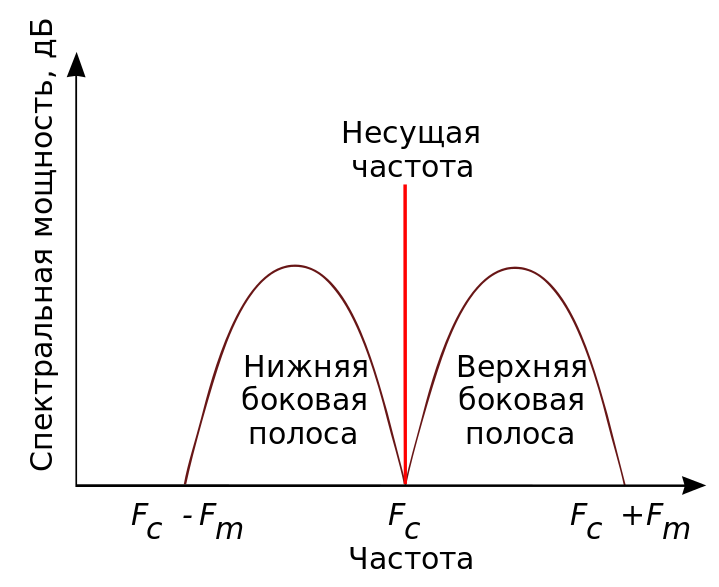
\includegraphics[scale=0.7]{spec_an_mod_theor}
		\caption{Спектр амплитудно-модулированного сигнала} 
		\label{pic:spec_an_mod_theor} % название для ссылок внутри кода
	\end{center}
\end{figure}

\subsubsection{Амплитудная модуляция с подавлением несущей}
Основная доля мощности АМ – сигнала приходится на несущую частоту. При \textit{балансной модуляции} (или АМ с подавлением несущей частоты (АМ-ПН) производится перемножение двух сигналов – модулирующего и несущего, при котором происходит подавление несущего колебания, соответственно, КПД модуляции становится равным 100\%. Формула для балансной модуляции:
\begin{equation}
	u(t) = M U_m cos(\Omega t) cos(\omega_0 t + \varphi _0)
\end{equation}
Спектр балансно-модулированного сигнала представлен на Рис.\ref{pic:spec_an_mod_carrier_theor}:
\begin{figure}[H]
	\begin{center}
		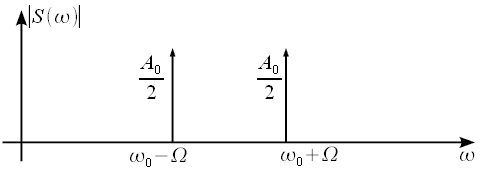
\includegraphics[scale=0.7]{spec_an_mod_carrier_theor}
		\caption{Спектр балансно-модулированного сигнала} 
		\label{pic:spec_an_mod_carrier_theor} % название для ссылок внутри кода
	\end{center}
\end{figure}

\subsubsection{Однополосная модуляция}
При идентичности информации в группах верхних и нижних боковых частот нет необходимости в их одновременной передаче. Одна из них перед подачей сигнала в канал связи может быть удалена, чем достигается двукратное сокращение полосы занимаемых сигналом частот. Уравнение сигнала с одной боковой полосой (ОБП – сигнал, \textit{single side band} – SSB) приведено ниже:
 \begin{equation}
	u(t) = U_m cos(\Omega t) cos(\omega_0 t + \varphi _0) + \frac{U_m}{2} \sum_{n=1}^{N}  M_n cos((\omega_0 + \Omega_n) t + \varphi _0 + \Phi _n)
\end{equation}
Внешняя форма ОБП – сигнала сходна с обычным АМ – сигналом, но ее огибающая имеет в два раза меньшую амплитуду по сравнению с АМ при М = 1. Для демодуляции ОБП – сигнала может использоваться как двухполупериодное, так и синхронное детектирование, со всеми особенностями, присущими этим методам. Результаты демодуляции отличаются от демодуляции АМ – сигналов только в два раза меньшей амплитудой выходных сигналов.

Спектр однополосно-модулированного сигнала и структурная схема соответствующего устройства представлены на Рис.\ref{pic:spec_an_mod_singleband_theor}:
\begin{figure}[H]
	\begin{center}
		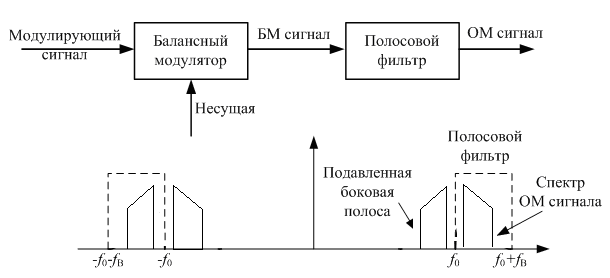
\includegraphics[scale=0.7]{spec_an_mod_singleband_theor}
		\caption{Спектр однополосно-модулированного сигнала} 
		\label{pic:spec_an_mod_singleband_theor} % название для ссылок внутри кода
	\end{center}
\end{figure}

\subsubsection{Демодуляция с помощью синхронного детектирования}
При синхронном детектировании модулированный сигнал умножается на опорное колебание с частотой несущего колебания:
 \begin{equation}
	y(t) = U(t) cos(\omega_0 t) cos(\omega_0 t) = \frac{U(t)}{2} (1 + cos(2\omega_0 t))
\end{equation}
Сигнал разделяется на два слагаемых, первое из которых повторяет исходный модулирующий сигнал, а второе повторяет модулированный сигнал на удвоенной несущей частоте 2$\omega_0$. Форма новой несущей при синхронном детектировании является чистой гармоникой, в отличие от двухполупериодного детектирования, где новая несущая содержит дополнительные гармоники более высоких частот. 

Физический амплитудный спектр сигналов после демодуляции подобен спектру двухполупериодного детектирования, но однозначно соотносится со спектром входного модулированного сигнала: амплитуды гармоник модулированного сигнала на частоте 2$\omega_0$ в два раза меньше амплитуд входного сигнала, постоянная составляющая равна амплитуде несущей частоты $\omega_0$ и не зависит от глубины модуляции, амплитуда информационного демодулированного сигнала в два раза меньше амплитуды исходного модулирующего сигнала. 

Особенностью синхронного детектирования является независимость от глубины модуляции, т.е. коэффициент модуляции сигнала может быть больше единицы. При синхронном детектировании требуется точное совпадение фаз и частот опорного колебания демодулятора и несущей гармоники АМ-сигнала.

\subsubsection{КПД модуляции}
КПД амплитудной модуляции зависит от коэффициента модуляции и может быть расчитано по следующей формуле:
 \begin{equation}
	\eta (t) =\frac{ U_m^2(t) M^2}{4 P_U}  = \frac{M^2}{2 + M^2} 
\end{equation}



\section{Ход работы}
Код программы представлен ниже \ref{code:code_1}:
\lstinputlisting[
	label=code:code_1,
	caption={Код в МатЛаб},% для печати символ '_' требует выходной символ '\'
]{Code_1.m}
В коде применены функции ammod и ssbmod.

\subsection{Генерация однотонального сигнала}
Для начала получим обычный гармонический сигнал. Сгенерированный сигнал представлен на рисунке \ref{pic:signal_one_tone}:
\begin{figure}[H]
	\begin{center}
		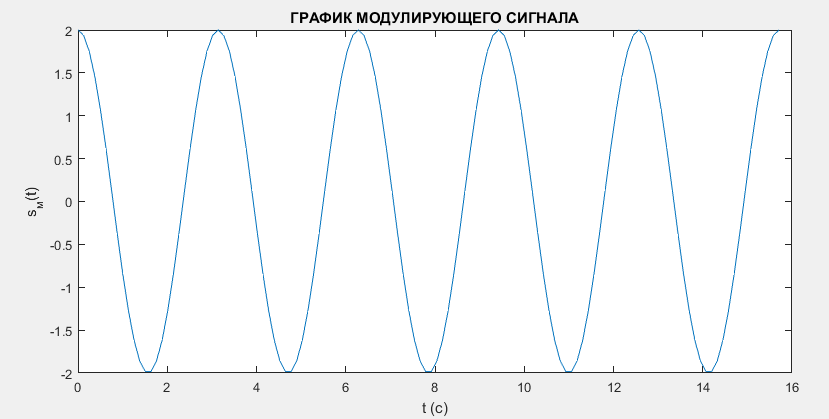
\includegraphics[scale=0.7]{signal_one_tone}
		\caption{Гармонический сигнал $s(t) = A*cos(2*\pi * f*t + \varphi)$} 
		\label{pic:signal_one_tone} % название для ссылок внутри кода
	\end{center}
\end{figure}
Для однотонального сигнала спектр выглядит следующим образом:
\begin{figure}[H]
	\begin{center}
		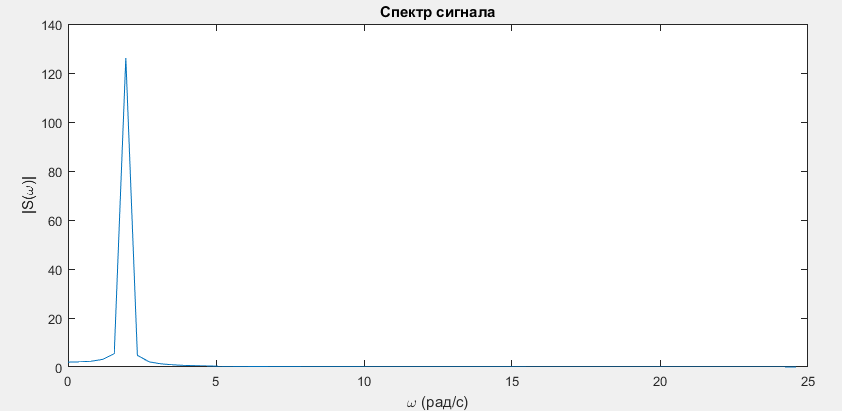
\includegraphics[scale=0.7]{signal_one_tone_spec}
		\caption{Спектр гармонического сигнала $s(t) = A*cos(2*\pi * f*t + \varphi)$} 
		\label{pic:signal_one_tone_spec} % название для ссылок внутри кода
	\end{center}
\end{figure}

\subsection{Амплитудная модуляция}
Сгенерированный однотональный сигнал подвергли амплитудной модуляции (при соотношении амплитуд инф./несущ. = 0.5). Сигнал после модуляции и его спектр представлены на рисунках \ref{pic:signal_modulated_0_5} и \ref{pic:mod_sig_spec_0_5}:
\begin{figure}[H]
	\begin{center}
		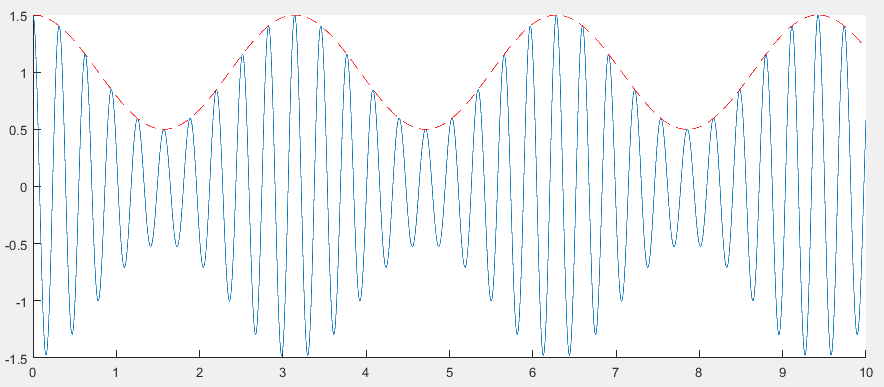
\includegraphics[scale=0.7]{signal_modulated_0_5}
		\caption{Амплитудно-модулированный сигнал ($M = 0.5$)} 
		\label{pic:signal_modulated_0_5} % название для ссылок внутри кода
	\end{center}
\end{figure}

\begin{figure}[H]
	\begin{center}
		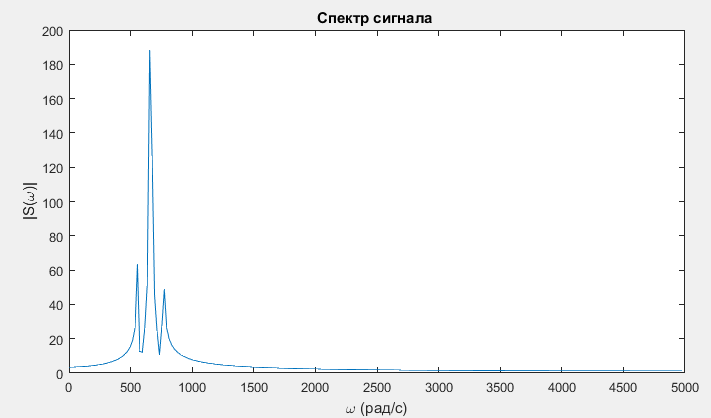
\includegraphics[scale=0.7]{mod_sig_spec_0_5}
		\caption{Спектр амплитудно-модулированного сигнала ($M = 0.5$)} 
		\label{pic:mod_sig_spec_0_5} % название для ссылок внутри кода
	\end{center}
\end{figure}
Спектр содержит гармонику модулирующего (информационного) сигнала и две гармоники по бокам - модулируемого (несущего).

Теперь будем изменять амплитуду модулирующего (информационного) сигнала для наблюдения изменения сигнала с модуляцией (его коэффициента модуляции M).

Пусть $M = 0.2$.
\begin{figure}[H]
	\begin{center}
		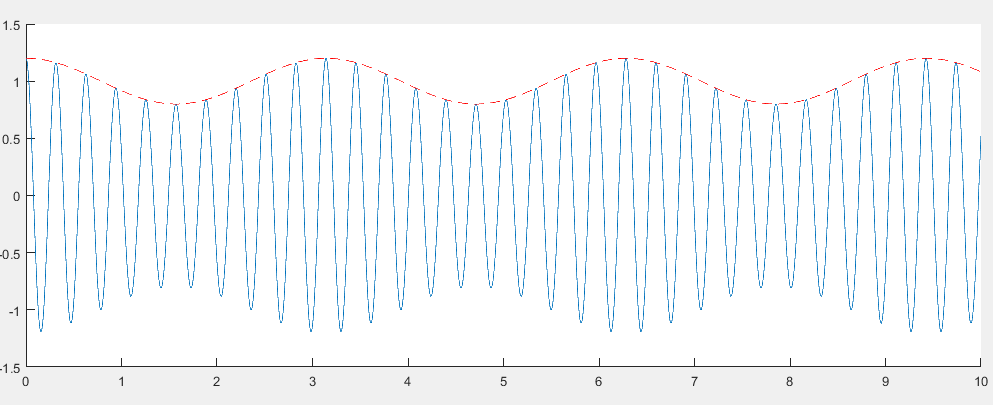
\includegraphics[scale=0.7]{signal_modulated_0_2}
		\caption{Амплитудно-модулированный сигнал ($M = 0.2$)} 
		\label{pic:signal_modulated_0_2} % название для ссылок внутри кода
	\end{center}
\end{figure}
\begin{figure}[H]
	\begin{center}
		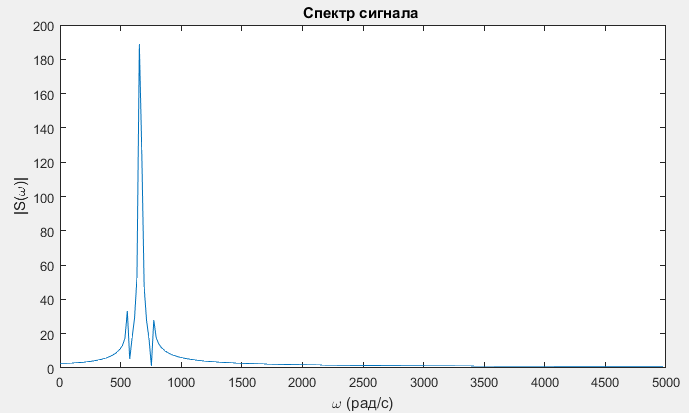
\includegraphics[scale=0.7]{mod_sig_spec_0_2}
		\caption{Спектр амплитудно-модулированного сигнала ($M = 0.2$)} 
		\label{pic:mod_sig_spec_0_2} % название для ссылок внутри кода
	\end{center}
\end{figure}

Пусть $M = 1$.
\begin{figure}[H]
	\begin{center}
		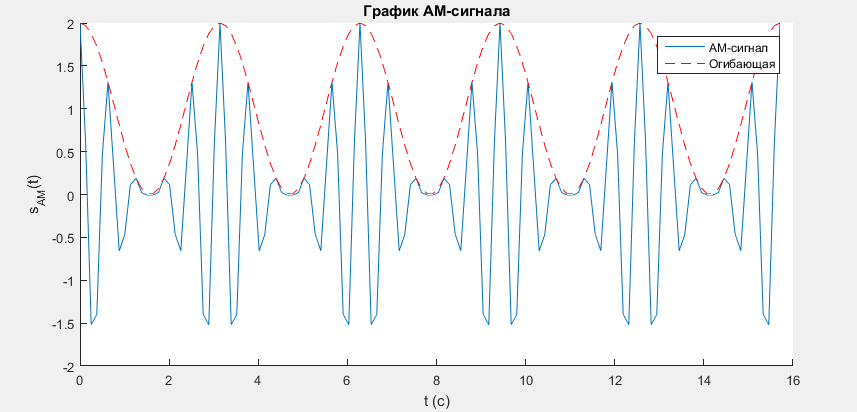
\includegraphics[scale=0.7]{signal_modulated_1_0}
		\caption{Амплитудно-модулированный сигнал ($M = 1$)} 
		\label{pic:signal_modulated_1_0} % название для ссылок внутри кода
	\end{center}
\end{figure}
\begin{figure}[H]
	\begin{center}
		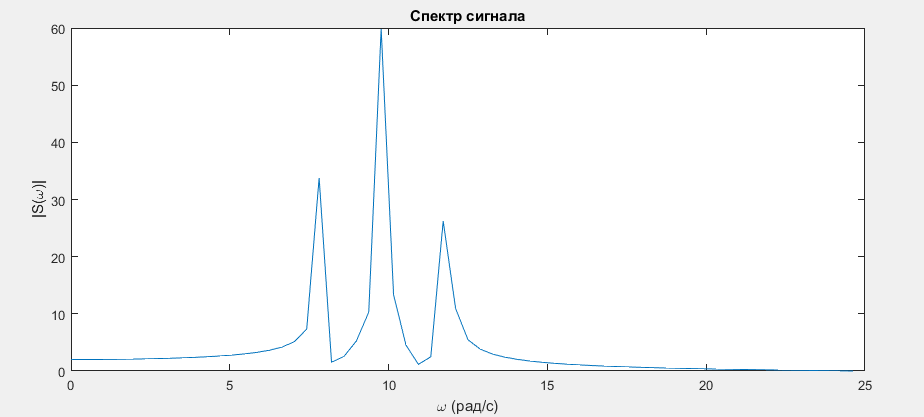
\includegraphics[scale=0.7]{mod_sig_spec_1_0}
		\caption{Спектр амплитудно-модулированного сигнала ($M = 1$)} 
		\label{pic:mod_sig_spec_1_0} % название для ссылок внутри кода
	\end{center}
\end{figure}

Пусть $M = 2$.
\begin{figure}[H]
	\begin{center}
		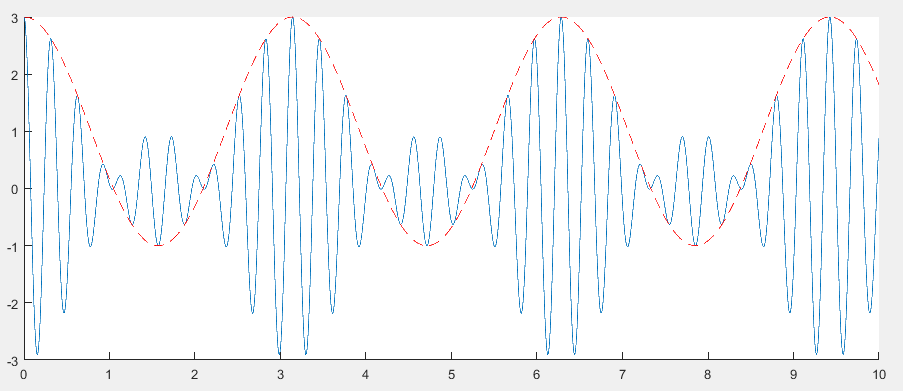
\includegraphics[scale=0.7]{signal_modulated_2_0}
		\caption{Амплитудно-модулированный сигнал ($M = 2$)} 
		\label{pic:signal_modulated_2_0} % название для ссылок внутри кода
	\end{center}
\end{figure}
\begin{figure}[H]
	\begin{center}
		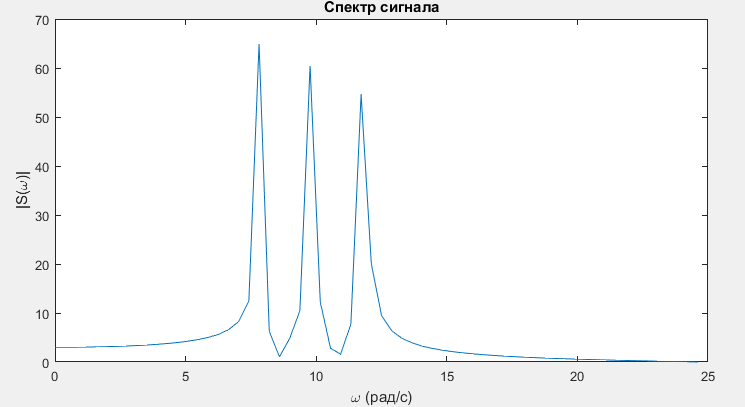
\includegraphics[scale=0.7]{mod_sig_spec_2_0}
		\caption{Спектр амплитудно-модулированного сигнала ($M = 2$)} 
		\label{pic:mod_sig_spec_2_0} % название для ссылок внутри кода
	\end{center}
\end{figure}

Пусть $M = 5$.
\begin{figure}[H]
	\begin{center}
		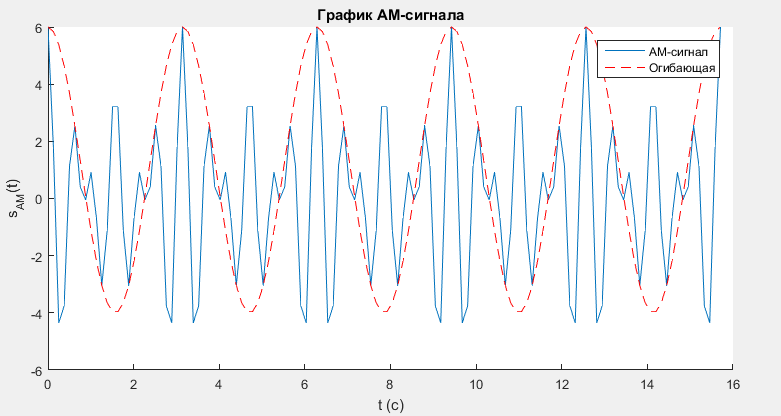
\includegraphics[scale=0.7]{signal_modulated_5_0}
		\caption{Амплитудно-модулированный сигнал ($M = 5$)} 
		\label{pic:signal_modulated_5_0} % название для ссылок внутри кода
	\end{center}
\end{figure}
\begin{figure}[H]
	\begin{center}
		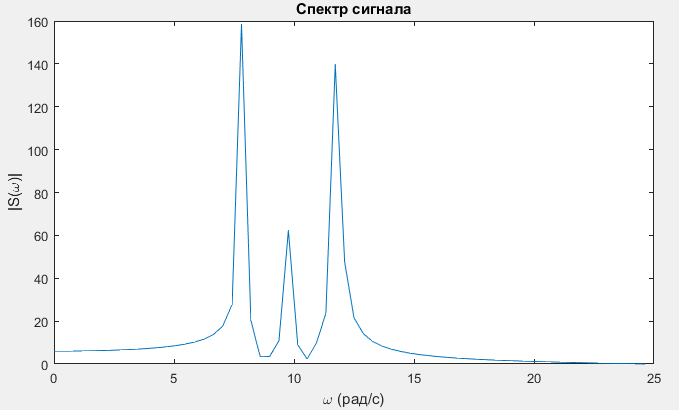
\includegraphics[scale=0.7]{mod_sig_spec_5_0}
		\caption{Спектр амплитудно-модулированного сигнала ($M = 5$)} 
		\label{pic:mod_sig_spec_5_0} % название для ссылок внутри кода
	\end{center}
\end{figure}
При M > 1 имеем случай перемодуляции, при M = 1 - случай глубокой модуляции, а при M < 1 - обычный случай модуляции без совмещений полупериодов гармонического сигнала огибающей.

\subsection{Амплитудная модуляция с подавлением несущей}
Подавление несущей осуществляется узкополосной фильтрацией сигнала на частоте информационного. Сигнал с АМ-ПН представлен на рисунке \ref{pic:signal_mod_carrier}:
\begin{figure}[H]
	\begin{center}
		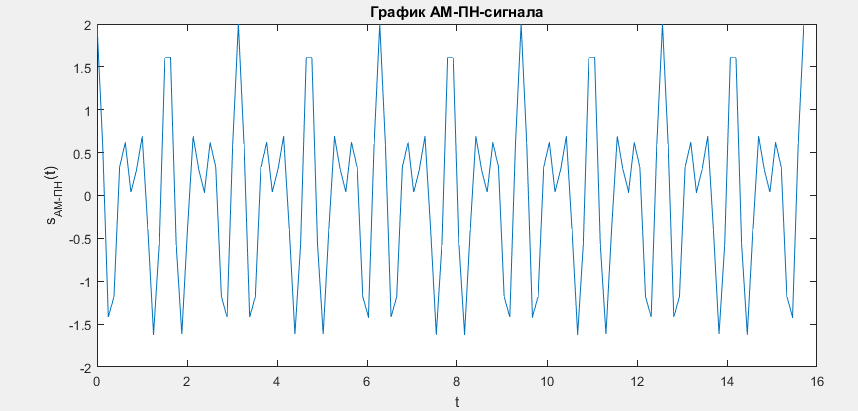
\includegraphics[scale=0.7]{signal_mod_carrier}
		\caption{Сигнал с АМ-ПН} 
		\label{pic:signal_mod_carrier} % название для ссылок внутри кода
	\end{center}
\end{figure}
Подавление несущей приводит к тому, что основная мощность сигнала (приходящаяся на несущую гармонику) фильтруется, но такой сигнал не демодулируется. Решить такую проблему можно частичной фильтрацией несущей, то есть сохранение амплитуды этой гармоники ненулевой, но более низкой, чем у информационной составляющей.

\subsection{Однополосная амплитудная модуляция}
Помимо подавления несущей, можно избавиться от лишней (дублирующейся) боковой полосы спектра с помощью ФНЧ. Сигнал с АМ-ОП представлен на рисунке \ref{pic:signal_mod_singleband}:
\begin{figure}[H]
	\begin{center}
		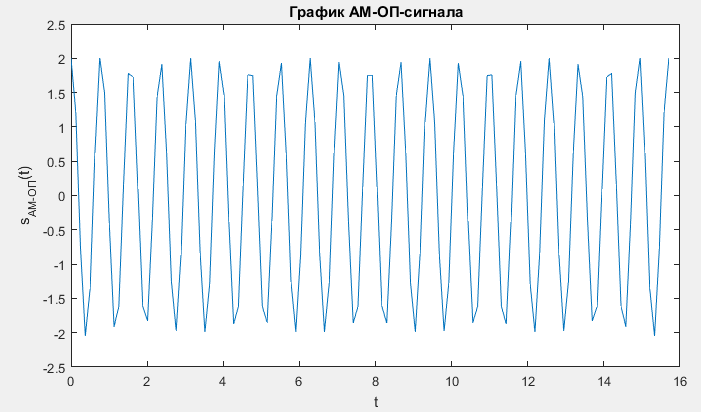
\includegraphics[scale=0.7]{signal_mod_singleband}
		\caption{Сигнал с АМ-ОП} 
		\label{pic:signal_mod_singleband} % название для ссылок внутри кода
	\end{center}
\end{figure}

\subsection{Спектры АМ-ПН и АМ-ОП}
Ниже, на рисунке \ref{pic:signal_mod_carrier_sinband_specs}, приведены спектры сигналов после АМ-ПН и АМ-ОП.
\begin{figure}[H]
	\begin{center}
		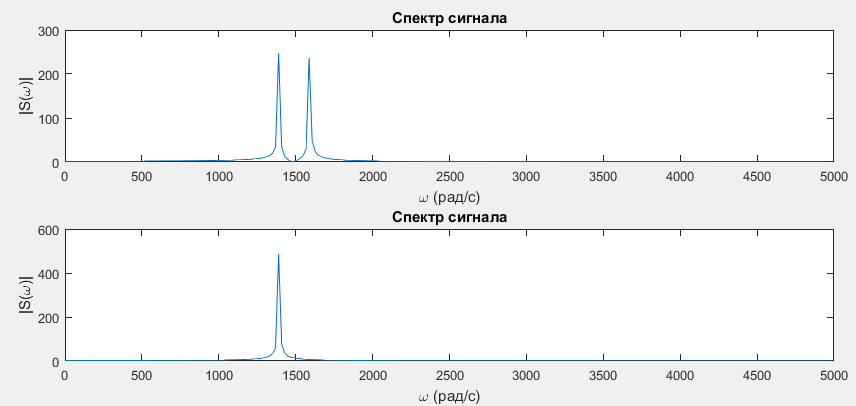
\includegraphics[scale=0.7]{signal_mod_carrier_sinband_specs}
		\caption{Спектры сигнала с АМ-ПН и АМ-ОП} 
		\label{pic:signal_mod_carrier_sinband_specs} % название для ссылок внутри кода
	\end{center}
\end{figure}
На первом рисунке видны две полосы (без несущей), что соответствует АМ-ПН. Ниже приведён спектр, содержащий одну полосу, что соответствует АМ-ОП.

\subsection{Демодуляция с помощью синхронного детектирования}
Произведем демодуляцию модулированных сигналов с разными коэффициентами модуляции.

Пусть $M = 0.2$.
\begin{figure}[H]
	\begin{center}
		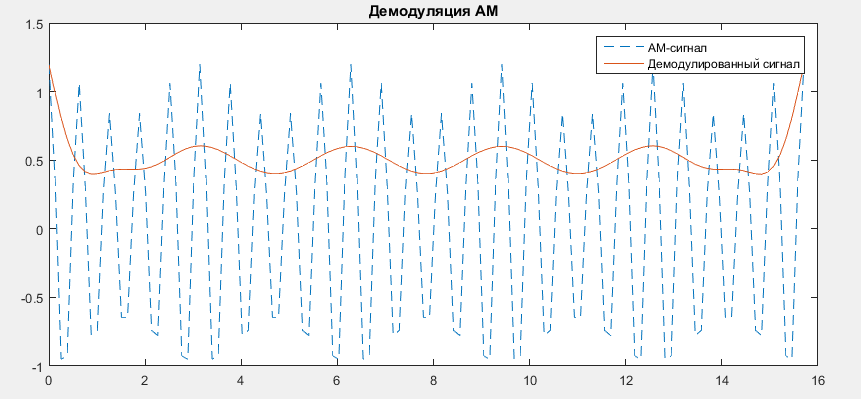
\includegraphics[scale=0.7]{sig_demod_0_2}
		\caption{Демодулированный сигнал ($M = 0.2$)} 
		\label{pic:sig_demod_0_2} % название для ссылок внутри кода
	\end{center}
\end{figure}

Пусть $M = 0.5$.
\begin{figure}[H]
	\begin{center}
		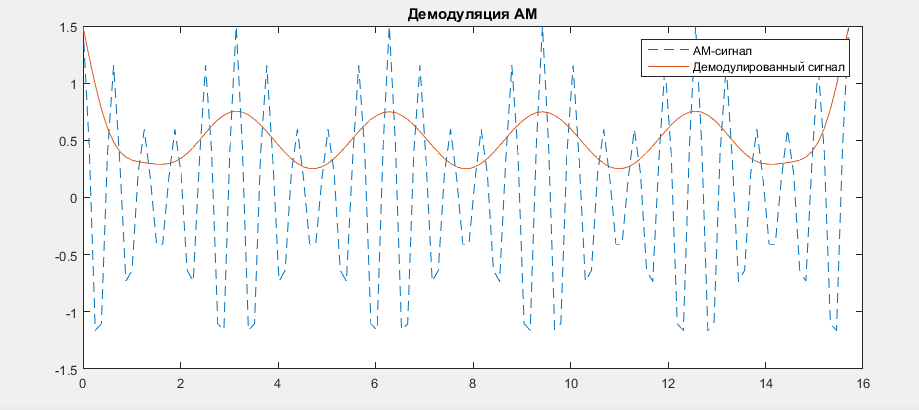
\includegraphics[scale=0.7]{sig_demod_0_5}
		\caption{Амплитудно-модулированный сигнал ($M = 0.5$)} 
		\label{pic:sig_demod_0_5} % название для ссылок внутри кода
	\end{center}
\end{figure}

Пусть $M = 1$.
\begin{figure}[H]
	\begin{center}
		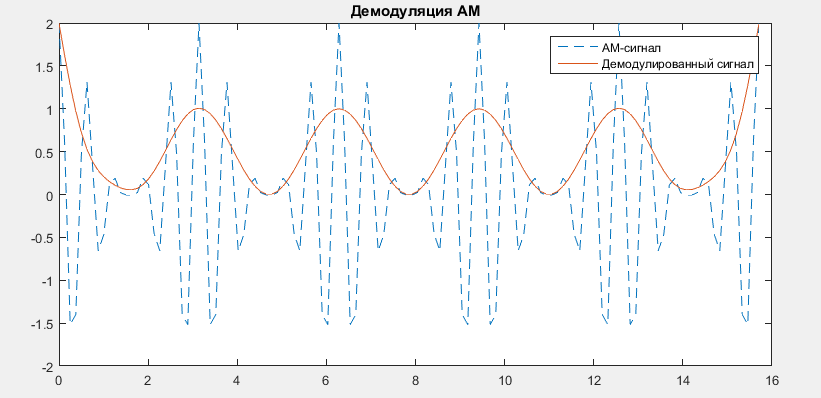
\includegraphics[scale=0.7]{sig_demod_1_0}
		\caption{Амплитудно-модулированный сигнал ($M = 1$)} 
		\label{pic:sig_demod_1_0} % название для ссылок внутри кода
	\end{center}
\end{figure}

Пусть $M = 2$.
\begin{figure}[H]
	\begin{center}
		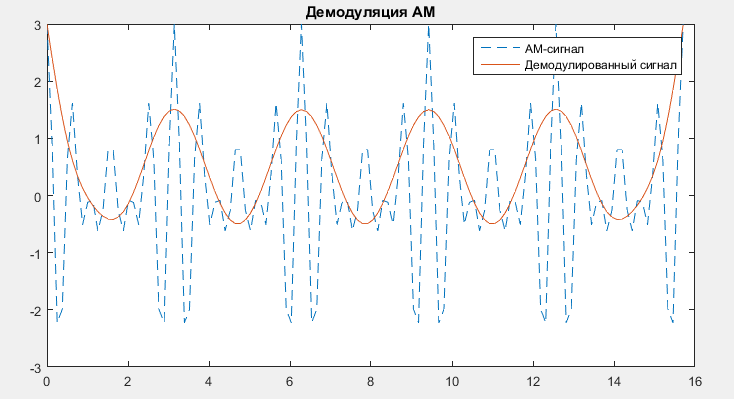
\includegraphics[scale=0.7]{sig_demod_2_0}
		\caption{Амплитудно-модулированный сигнал ($M = 2$)} 
		\label{pic:sig_demod_2_0} % название для ссылок внутри кода
	\end{center}
\end{figure}

Пусть $M = 5$.
\begin{figure}[H]
	\begin{center}
		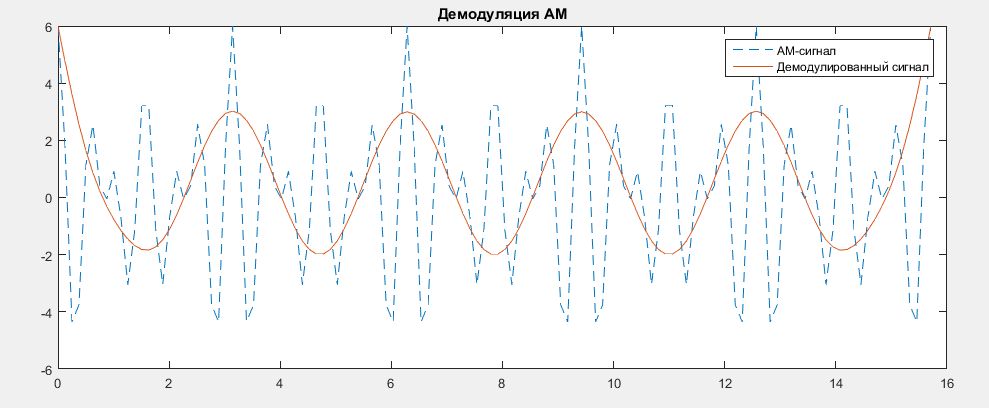
\includegraphics[scale=0.7]{sig_demod_5_0}
		\caption{Амплитудно-модулированный сигнал ($M = 5$)} 
		\label{pic:sig_demod_5_0} % название для ссылок внутри кода
	\end{center}
\end{figure}
Как можно видеть, нелинейные искажения сигнала при демодуляции тем незначительнее, чем больше коэффициент модуляции.
Ниже приведен спектр демодулированного сигнала при M = 2.
\begin{figure}[H]
	\begin{center}
		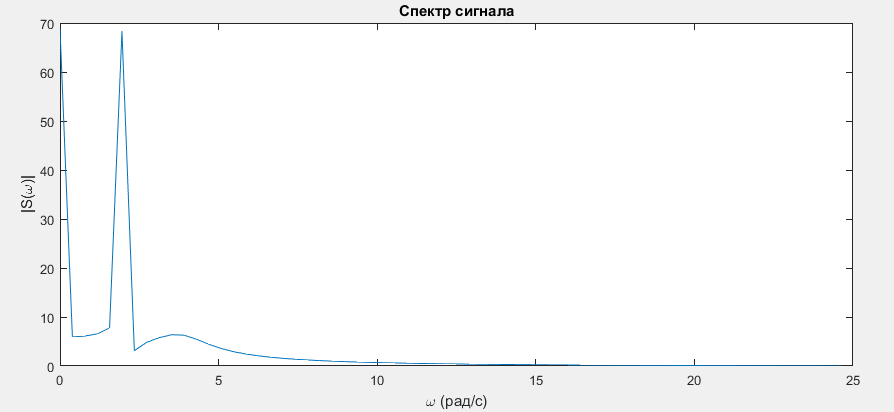
\includegraphics[scale=0.7]{sig_demod_spec_2_0}
		\caption{Спектр демодулированного сигнала ($M = 2$)} 
		\label{pic:sig_demod_spec_2_0} % название для ссылок внутри кода
	\end{center}
\end{figure}
В сигнале появились низкочастотная составляющая и высокочастотные искажения, однако при применении полосового фильтра можно выделить искомый сигнал с достаточной точностью совпадающий с исходным.

При M = 5 имеем:
\begin{figure}[H]
	\begin{center}
		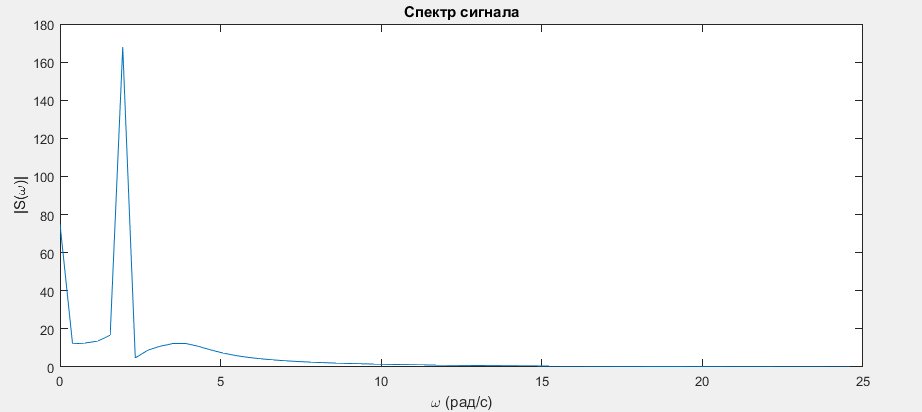
\includegraphics[scale=0.7]{sig_demod_spec_5_0}
		\caption{Спектр демодулированного сигнала ($M = 5$)} 
		\label{pic:sig_demod_spec_5_0} % название для ссылок внутри кода
	\end{center}
\end{figure} 
Низкочастотная составляющая значительно меньше по амплитуде, чем информационная, высокочастотные искажения так же стали более незначительны, чем при M = 2.

\subsection{КПД модуляции}
Ниже, на рисунке \ref{pic:Kpd_ampmod}, приведена зависимость КПД модуляции от амплитуды модулирующего сигнала (т.е. от коэффициента модуляции).
\begin{figure}[H]
	\begin{center}
		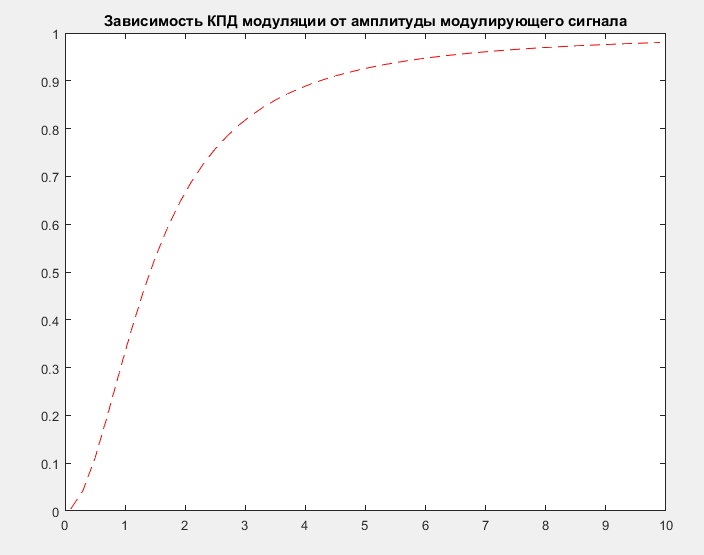
\includegraphics[scale=0.7]{Kpd_ampmod}
		\caption{Спектры сигнала с АМ-ПН и АМ-ОП} 
		\label{pic:Kpd_ampmod} % название для ссылок внутри кода
	\end{center}
\end{figure}

\section{Выводы}

Исследованы типы аналоговой модуляции (амплитудная, с подавлением несущей и однополосная), также исследован способ демодуляции с помощью синхронного детектирования и определена зависимость КПД модуляции от коэффициента модуляции. Построены спектры модулированных сигналов, их вид совпал с ожидаемым результатом для каждого типа модуляции.

Основной результат данного исследования - получение представления об эффективности и принципах аналоговой амплитудной модуляции. Она находит широкое применение: в системах телевизионного вещания (для передачи телевизионных сигналов), в системах звукового радиовещания и радиосвязи на длинных и средних волнах,
в системе трехпрограммного проводного вещания.

\end{document}
